% Configuration
\documentclass[11pt,a4paper]{article}
\usepackage[numbers]{natbib}
\usepackage[french]{babel}
\usepackage[utf8]{inputenc}
\usepackage[T1]{fontenc}
\usepackage{mathptmx}   % Times New Roman

\usepackage{xcolor}
\definecolor{bleu}{RGB}{0,113,185}
\definecolor{white}{RGB}{255,255,255}
\definecolor{black}{RGB}{0,0,0}

\usepackage{setspace}
\usepackage{afterpage}
\usepackage[a4paper,top=4cm,bottom=3cm,left=3cm,right=3cm,marginparwidth=1.75cm]{geometry}
\usepackage{fancyhdr}

\usepackage{amsmath,amsthm,amssymb,amsfonts}
\usepackage{graphicx}
\usepackage{color}
\usepackage[colorlinks=false]{hyperref}
\usepackage{float}

\usepackage{tabularx}      % Pour ajuster la largeur du tableau
\usepackage[table]{xcolor} % Pour les couleurs de cellules/lignes

% Saut de page après chaque section

\usepackage{fancyhdr}
\usepackage{titlesec}
\newcommand{\sectionbreak}{\clearpage}

% Configuration des listes

\usepackage{enumitem}
\setlist{
    itemsep=0.1em,    % Espace entre les éléments de la liste
    topsep=0.1em,     % Espace avant la liste
    parsep=0.3em,     % Espace entre les paragraphes à l'intérieur d'un item
    after=\vspace{1em}       % Espace après la liste
}

% Mise en page

\renewcommand{\baselinestretch}{1}
\setlength{\parindent}{10pt}
\setlength{\parskip}{0.8em}

% Informations du fichier

\title{PADR}
\author{Malo Goossens}

%Informations destinées à la couverture

\newcommand{\titre}{Programmation d'applications distribuées en réseau}
\newcommand{\auteur}{Malo Goossens}
\newcommand{\prof}{Dr. Laurent Philippe, M. Adrien Huygens}
\newcommand{\master}{Master 1 en Architecture des Systèmes Informatiques}
\newcommand{\annee}{Année académique  2025-2026}

% --------------------------------

\pagestyle{fancy}
\fancyhead{}
\fancyfoot{}
\renewcommand{\headrulewidth}{0pt}
\fancyfoot[R]{\thepage}

\begin{document}
\thispagestyle{empty}
\pagecolor{bleu}\afterpage{\nopagecolor}

\begin{center}

\includegraphics[width=7cm]{figures/logos.png}	% Pour inclure le logo (on précise la largeur de l'image)
\end{center}

\vspace{3cm}
\begin{center}
{\huge \color{white} \sf \titre}
\vspace{2cm}
\\ {\color{white} \sf \Large  \auteur}

\vspace{4cm}
\begin{center}
{\color{white} \noindent\rule{2cm}{0.4pt}}
\end{center}
\vspace{1cm}
{\color{white} \sf \Large  \prof}
\vspace{1cm}
\\ {\color{white} \sf  \small  \master}
\\ {\color{white} \sf  \small  \annee}
\pagebreak

\end{center}

% Table des matières

\thispagestyle{empty}%
\tableofcontents
\vfill\cleardoublepage%

% Contenu du document

% Bibliographie

\bibliographystyle{ieeetr} 
\renewcommand\refname{Bibliographie}

\section*{Introduction}
L'objectif de ce projet est de concevoir un système de résolution de noms de domaine (DNS).
Cette implémentation doit se faire en python et à partir de zéro, sans utiliser de bibliothèques spécialisées.
Chaque serveur du système doit être capable de résoudre les requêtes DNS de manière récursive et posséder un cache en plus de gérer l'éventuelle zone dont elle serait responsable.

Ce projet à réaliser par équipe de 1 étudiant, demande d'appliquer la méthodologie de gestion de projet \textit{Agile} pour la conception et l'implémentation du système DNS.
En particulier, il est demandé d'implémenter des tests unitaires pour valider le bon fonctionnement du système et garantir la qualité du code produit.
Les artéfacts produits au cours du projet sont constatables sur le dépôt GitLab~\cite{gitlab_dns_project} et sont constitués de la documentation, du code source et des tests unitaires.

Le présent rapport décrit la conception et l'implémentation de ce système DNS.
Il commencera par une analyse du contexte et du cahier des charges, suivie d'une analyse fonctionnelle listant les besoins et les contraintes du système.
L'analyse technique détaillera ensuite l'architecture logicielle et les choix de conception.
Enfin, la section sur l'implémentation et la validation présentera les résultats des tests.

\subsection{Objectif du projet}
% TODO: Rédiger l'objectif global du projet.
% - Expliquer la démarche "from scratch" pour comprendre le DNS de l'intérieur.
% - Présenter la création des trois briques : Client CLI, Résolveur Récursif, Serveur Autoritaire.

\subsection{Périmètre et limites du système}
% TODO: Définir ce qui est implémenté et ce qui est exclu.
% - Inclus : Résolution itérative, gestion du cache, fallback TCP, réplication AXFR/NOTIFY, hot-reload.
% - Exclus : Signatures DNSSEC, interface graphique (GUI), support IPv6 avancé (si limité à l'IPv4).

\subsection{Organisation du document}
% TODO: Présenter rapidement le déroulé des chapitres suivants (Contexte, Analyse Fonctionnelle, Analyse Technique, Implémentation, Rétrospective, Note IAG).

\subsection{Le fonctionnement du protocole DNS}
% TODO: Présenter les principes fondamentaux du DNS.
% - La structure arborescente des noms de domaine.
% - La hiérarchie des serveurs : Root (.), TLD (.be), Serveurs Autoritaires.
% - La différence entre résolution récursive (vue client) et itérative (vue résolveur).

\subsection{La contrainte « Vanilla Python »}
% TODO: Expliquer les règles imposées pour ce projet.
% - Développement exclusivement avec la bibliothèque standard Python (struct, socket, threading, etc.).
% - Interdiction des bibliothèques tierces comme dnspython pour le cœur de protocole.
% % [À MENTIONNER]: L'absence de support POSIX natif sous Windows (notamment pour SIGHUP), imposant de trouver des mécanismes multiplateformes.

\subsection{L'interopérabilité et le respect de la RFC 1035}
% TODO: Développer les enjeux d'interopérabilité.
% - Nécessité de respecter scrupuleusement le format de trame binaire de 1987.
% - Garantir la compatibilité ascendante avec des outils système réels (dig, nslookup, host).

\section{Analyse fonctionnelle}
\subsection{Vision globale du système}
% TODO: Insérer et commenter le Schéma Conceptuel de l'infrastructure globale.
% \begin{figure}[htbp]
%   \centering
%   \include{diagrams/schema_conceptuel}
%   \caption{Architecture globale des flux entre le Client, le Résolveur et la Hiérarchie DNS.}
% \end{figure}
% - Expliquer le trajet d'une requête de bout en bout (Client -> Résolveur -> Racine -> TLD -> Autorité).

\subsection{Épic 1 : L'Outil Client (CLI)}
% TODO: Insérer le Use Case Diagram du Client.
% - Lister et détailler les US-1.1 à US-1.6 (envoi de requêtes, parsing d'arguments, affichage formaté).

\subsection{Épic 2 : Le Serveur Récursif (Le Chef d'orchestre)}
% TODO: Insérer le Use Case Diagram du Résolveur Récursif.
% - Lister et détailler les US-2.1 à US-2.7 (moteur itératif, cache, fallback TCP).
% - Explain administration feature: interception de la demande 'flush.cache.local' (TXT).
% % [À MENTIONNER]: Règle métier stricte : rejet systématique des requêtes reçues avec RD=0 via le code RCODE 5 (REFUSED).

\subsection{Épic 3 : Le Serveur d'Autorité (La Base de données)}
% TODO: Insérer le Use Case Diagram du NameServer.
% - Lister et détailler les US-3.1 à US-3.6 (chargement de zone, réponses autoritaires, hot-reload).

\subsection{Épics 4 et 5 : Tolérance aux pannes et Qualité}
% TODO: Présenter les fonctionnalités avancées.
% - Épic 4 (US-4.1 à US-4.5) : Mécanismes de réplication Master/Slave (AXFR et NOTIFY).
% - Épic 5 (US-5.1) : Exigences de qualité et couverture par tests unitaires.
\section{Analyse technique}
\subsection{Encodage et Sérialisation des données}
\subsubsection{La Forge des Messages}
Le cœur du protocole DNS est son format de message permettant aux clients, résolveurs récursifs et serveurs de noms de communiquer.
Il est donc essentiel de simplifier au maximum la lecture, la création et la (dé)sérialisation de ces messages qui seront utiliser par chaques composants du système.

\begin{figure}[H]
    \centering
    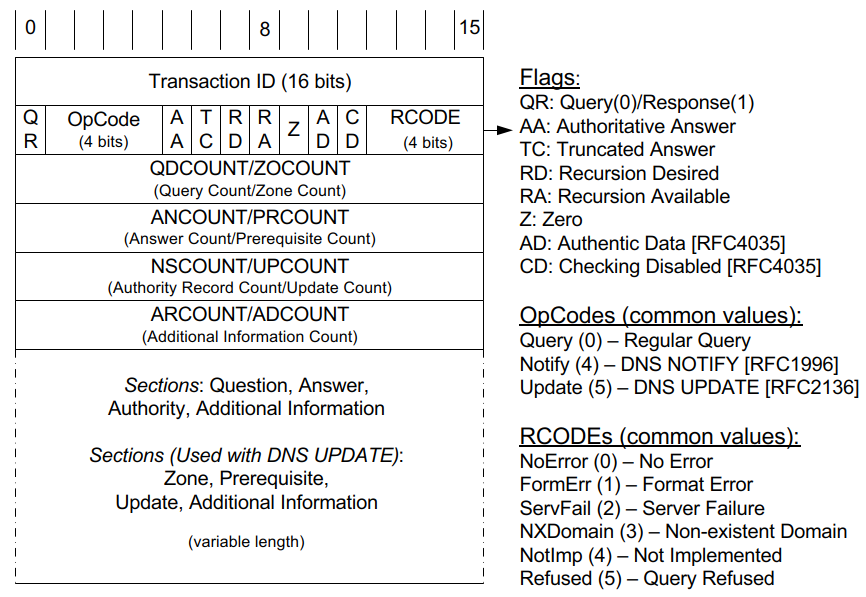
\includegraphics[width=15cm]{figures/technique/msg_format.png}
    \caption{Format des messages DNS~\cite{steven2012tcp}.}
    \label{fig:format_de_message}
\end{figure}

Comme illustré, le contenu d'un message DNS peut être séparé en sept sections.
Premièrement, un identifiant de transaction (encodé sur 16 bits) définit par le client et recopié par le serveur permet d'associer une requête à sa réponse.
La section suivant est un tampon de 16 bits constituants des drapeaux (flags) qui permettent de donner des informations sur la nature et l'état de la requête.
Ensuite, quatre nombres entiers (16 bits) donne le nombre d'entrées dans les sections suivantes, permettant ainsi de connaitre leur taille, ce qui est nécessaire pour les lire.
Finalement, la section query (question)
Les sections \texttt{question}, \texttt{answer}, \texttt{authority} et \texttt{additionnal} information, constituent le contenu du message.
Elles permettent respectivement de connaitre le type de données attendu, la réponse du serveur, les serveurs détenant la réponse et des informations complémentaires.

Les questions ont un format qui leur est propre, il est composé du nom de domaine concerné et du type de question qui est posé.
Les autres champs utilisent tous un format appelé \texttt{Resource Record} pour représenter les données transmises.
Ils sont composés d'un nom de domaine, de leur type (A, AAAA, NS, CNAME, TXT), de leur classe (toujours IN), du temps qu'ils doivent être conservés en cache (ttl) et de la donnée qu'ils contiennent au format binaire.
Les noms de domaines sont compressés par un algorithme qui évite d'encoder plusieurs fois les mêmes labels dans le message.

Ainsi, quatre classes python seront utilisées pour rendre la manipulation des messages transparente.
La classe \texttt{DNSMessage} contiendra les sept section présentés précédemment ainsi que les méthodes \texttt{pack} et \texttt{unpack} pour assurer la (dé)sérialisation.
Les classes \texttt{DNSQuestion} et \texttt{ResourceRequest} seront utilisées par \texttt{DNSMessage} pour représenter son contenu.
Le champ donné de \texttt{ResourceRecord} dépendant de son type, il est stocké au format binaire et est rendu accessible par une propriété qui le décode, à la demande, de la manière adéquate.
Enfin, la classe \texttt{DomainName} centralise la compression.

\begin{figure}[H]
    \centering
    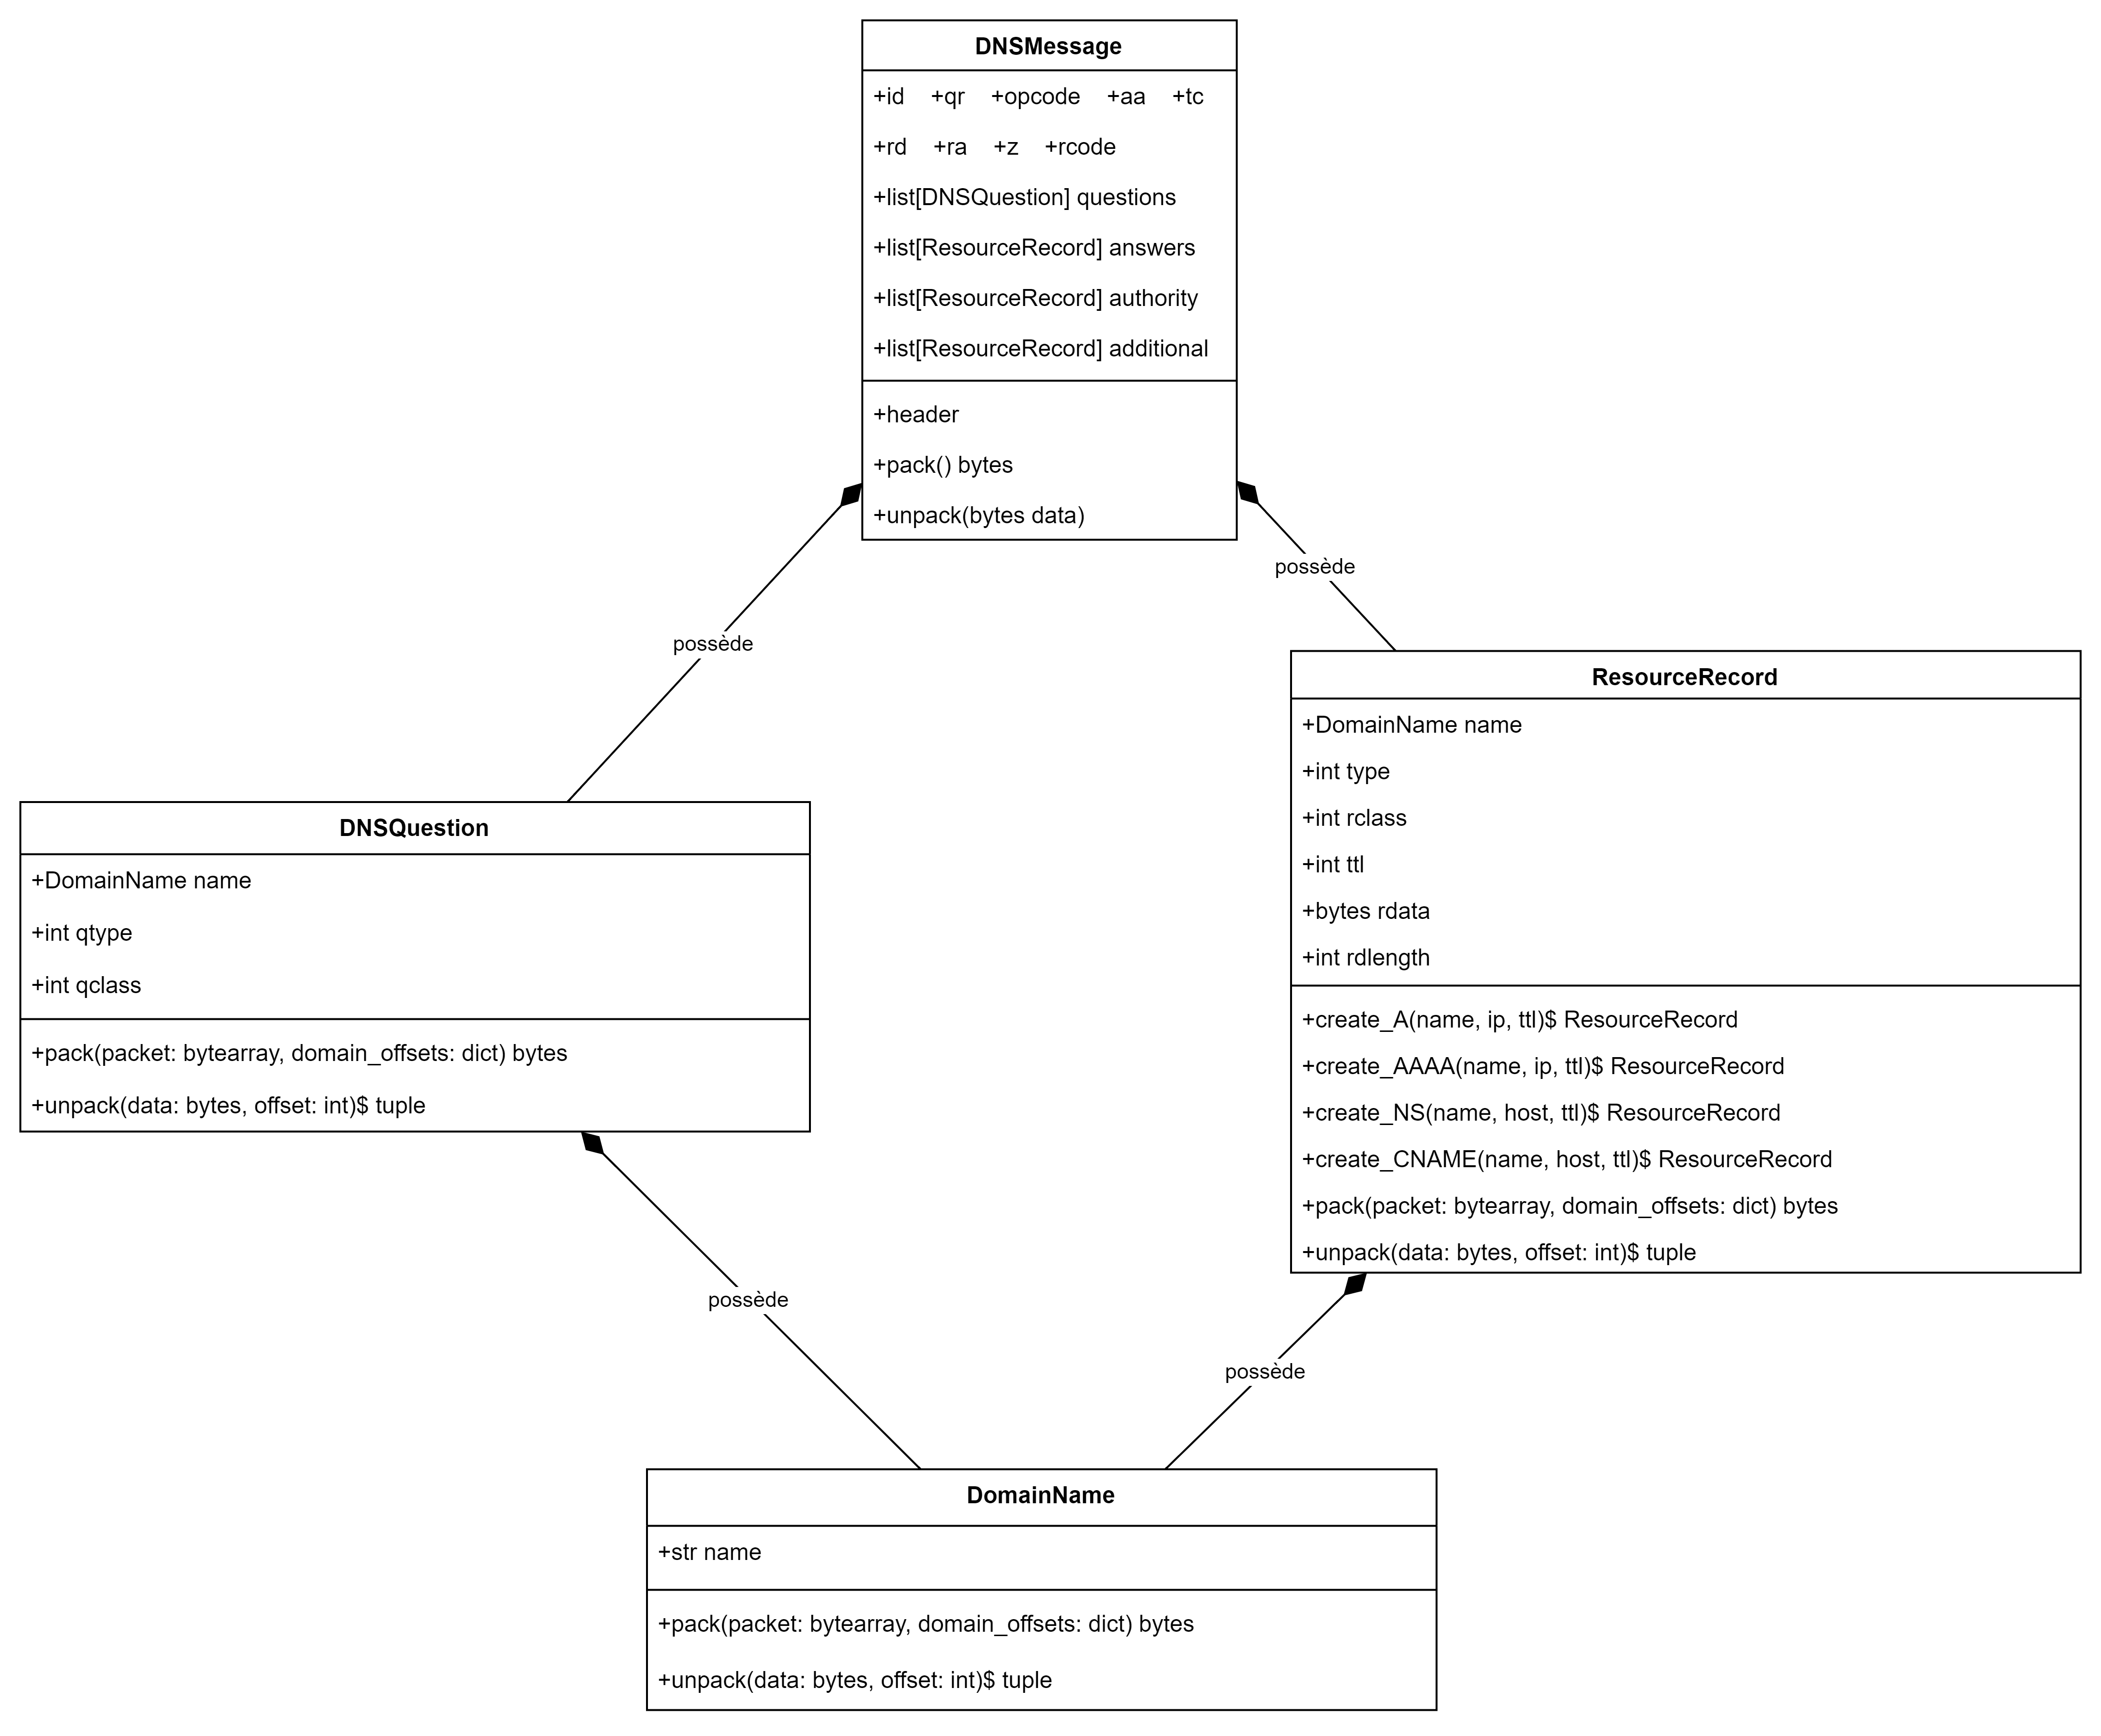
\includegraphics[width=15cm]{figures/technique/class_message.png}
    \caption{Diagramme de classe de la Forge à messages.}
    \label{fig:class_diagram_messages}
\end{figure}

\subsubsection{Encodage et masques bit-à-bit}
% TODO: Expliquer l'utilisation du module `struct` de Python (format '!HHHHHH').
% - Détailler la manipulation des flags d'en-tête (QR, Opcode, AA, TC, RD, RA, Rcode) via les décalages et masques binationaux.
Envoyer un message sur le réseau demande un contrôle de la couche binaire.
Python étant un langage de haut niveau, il est nécessaire de passer par le module \texttt{Struct}~\cite{python_doc_struct} pour atteindre cette granularité

\texttt{Struct} permet de convertir des types de données Python en flux d'octets et inversement.
Pour ce faire, il est nécessaire de définir un format de conversion.
Dans le cas de l'entête des messages DNS, le format de conversion est le suivant : \texttt{!HHHHHH}.
Le point d'exclamation indique que le flux d'octets est en big-endian.
Les six H indiquent que le flux contient six entiers non signés de 16 bits.
Les valeurs sont ensuite passées dans l'ordre de leur apparition dans l'entête.

Cette logique est utilisée par tous les objets qui doivent pouvoir être sérialisés (\texttt{DNSMessage}, \texttt{DNSQuestion}, \texttt{ResourceRecord}, \texttt{DomainName}).

\subsubsection{Compression des noms et gestion de la section ADDITIONAL}
% TODO: Expliquer le fonctionnement du pointeur de compression 0xC0.
% % [À MENTIONNER]: Gestion et tolérance de la section ADDITIONAL : ignorer silencieusement les enregistrements OPT (EDNS0, type 41) envoyés par dig/nslookup sans faire planter l'unpacking.
Un nom de domaine est composé de plusieurs labels séparés par des points.
Les labels sont lus de droite à gauche et chacun indique une sous-section de la zone définit par le précédent.

Les messages DNS contiennent souvent des domaines qui partagent des labels communs.
En l'absence de compression ces répétitions provoqueraient une perte de bande passante et de temps de traitement considérable à l'échelle d'internet.
Ainsi, à chaque fois qu'un label déjà présent dans le message doit être réutilisé, un pointeur de compression est utilisé à la place.
Le pointeur de compression est un entier de 16 bits dont les deux premiers bits sont à 1 et les 14 autres indiquent l'offset du label dans le message.

Le compte des labels déjà présents dans le message est tenu par un dictionnaire (clé = label, valeur = offset) créer dans la fonction \texttt{pack} de la classe \texttt{DNSMessage} et passé à la fonction \texttt{pack} de \texttt{DomainName} pour chaque nom de domaine à sérialiser.
À la lecture, une variable d'offset sert de tête de lecture pour savoir quel caractère est entrain d'être lu.
Lorsqu'un pointeur est détecté par les deux bits à 1, l'offset est mis à jour avec la valeur du pointeur et la lecture continue à partir de cette position jusqu'à la fin du nom de domaine.


\subsubsection{Encodage des enregistrements TXT}
% TODO: Développer le format spécifique des enregistrements TXT.
% % [À MENTIONNER]: Encodage Pascal-string des chaines TXT (1 octet de longueur + octets UTF-8) et vérification de la limite stricte des 255 octets par segment.
Contrairement aux adresses IP (types A et AAAA) qui ont une longueur fixe, les enregistrements de type TXT peuvent contenir des données textuelles de taille variable, souvent utilisées pour la vérification de domaine ou le filtrage anti-spam (SPF).
La norme RFC 1035 impose que ces chaînes de caractères soient encodées sous la forme de \texttt{Pascal-strings}. Ainsi, la donnée brute n'est pas simplement du texte encodé en UTF-8, mais doit systématiquement être préfixée par un octet indiquant la longueur de la chaîne qui suit.
De plus, ce format impose une contrainte stricte : un segment de texte ne peut excéder 255 octets.
Si un enregistrement TXT est plus long, il doit être découpé en plusieurs blocs successifs (longueur + données) au sein du même \texttt{Resource Record}.
Cette implémentation gère cette spécificité lors de la sérialisation pour garantir la compatibilité avec les clients standards.


\subsection{Architecture réseau}
% TODO: Séparation des responsabilités : DNSListener (socket serveur multi-threadé) vs DNSRequester (socket client).
% % [À MENTIONNER]: Décalage du port d'écoute hôte (10054 au lieu du port 53) pour contourner le verrouillage du service système Windows 'dnscache'.
\subsubsection{Stratégie Réseau (UDP vs TCP)}
Le protocole DNS repose historiquement sur le protocole UDP pour des raisons de vitesse.
En effet, l'absence de poignée de main (\texttt{handshake}) permet des résolutions extrêmement rapides.
Cependant, l'UDP étant sans connexion et non fiable, il limite la taille des messages à 512 octets.

Pour gérer les communications, l'architecture sépare strictement l'écoute (le serveur) et l'émission (le client).
La classe \texttt{DNSListener} ouvre des \texttt{sockets}\cite{python_doc_socket} serveurs multi-threadées (un thread par requête TCP) pour ne pas bloquer la réception des paquets.

À l'inverse, la classe \texttt{DNSRequester} gère l'émission avec des délais d'attente (\texttt{timeouts}) stricts pour éviter qu'un serveur distant silencieux ne bloque notre résolveur.

\subsubsection{Gestion du Fallback TCP}
% TODO: Détailler le passage d'UDP à TCP lorsque le bit TC (Truncated) est égal à 1.
% - Expliquer l'ajout du préfixe de longueur sur 2 octets en début de trame TCP (RFC 1035 section 4.2.2).
% - Insérer ici le Sequence Diagram : Fallback TCP.
Lorsqu'un serveur DNS doit renvoyer une réponse dépassant la limite des 512 octets en UDP (par exemple, une réponse contenant de multiples enregistrements de type AAAA ou de nombreuses signatures), il tronque le message et met le drapeau \texttt{TC} (\texttt{Truncated}) à 1 dans l'entête du message.
Notre résolveur implémente un mécanisme de \texttt{Fallback} transparent.
Ainsi, s'il détecte \texttt{TC=1}, il abandonne la réponse incomplète et initie immédiatement une nouvelle connexion TCP vers le même serveur.
La subtilité technique imposée par la RFC 1035 (section 4.2.2) réside dans l'encapsulation.
C'est-à-dire que sur un flux TCP (qui est continu, contrairement aux datagrammes UDP), chaque message DNS doit obligatoirement être préfixé par 2 octets indiquant la taille totale de la trame.
Notre classe \texttt{DNSRequester} gère l'ajout et le retrait de ce préfixe de manière transparente lors du basculement.

\subsubsection{Générisité de l'architecture}
\begin{figure}[H]
    \centering
    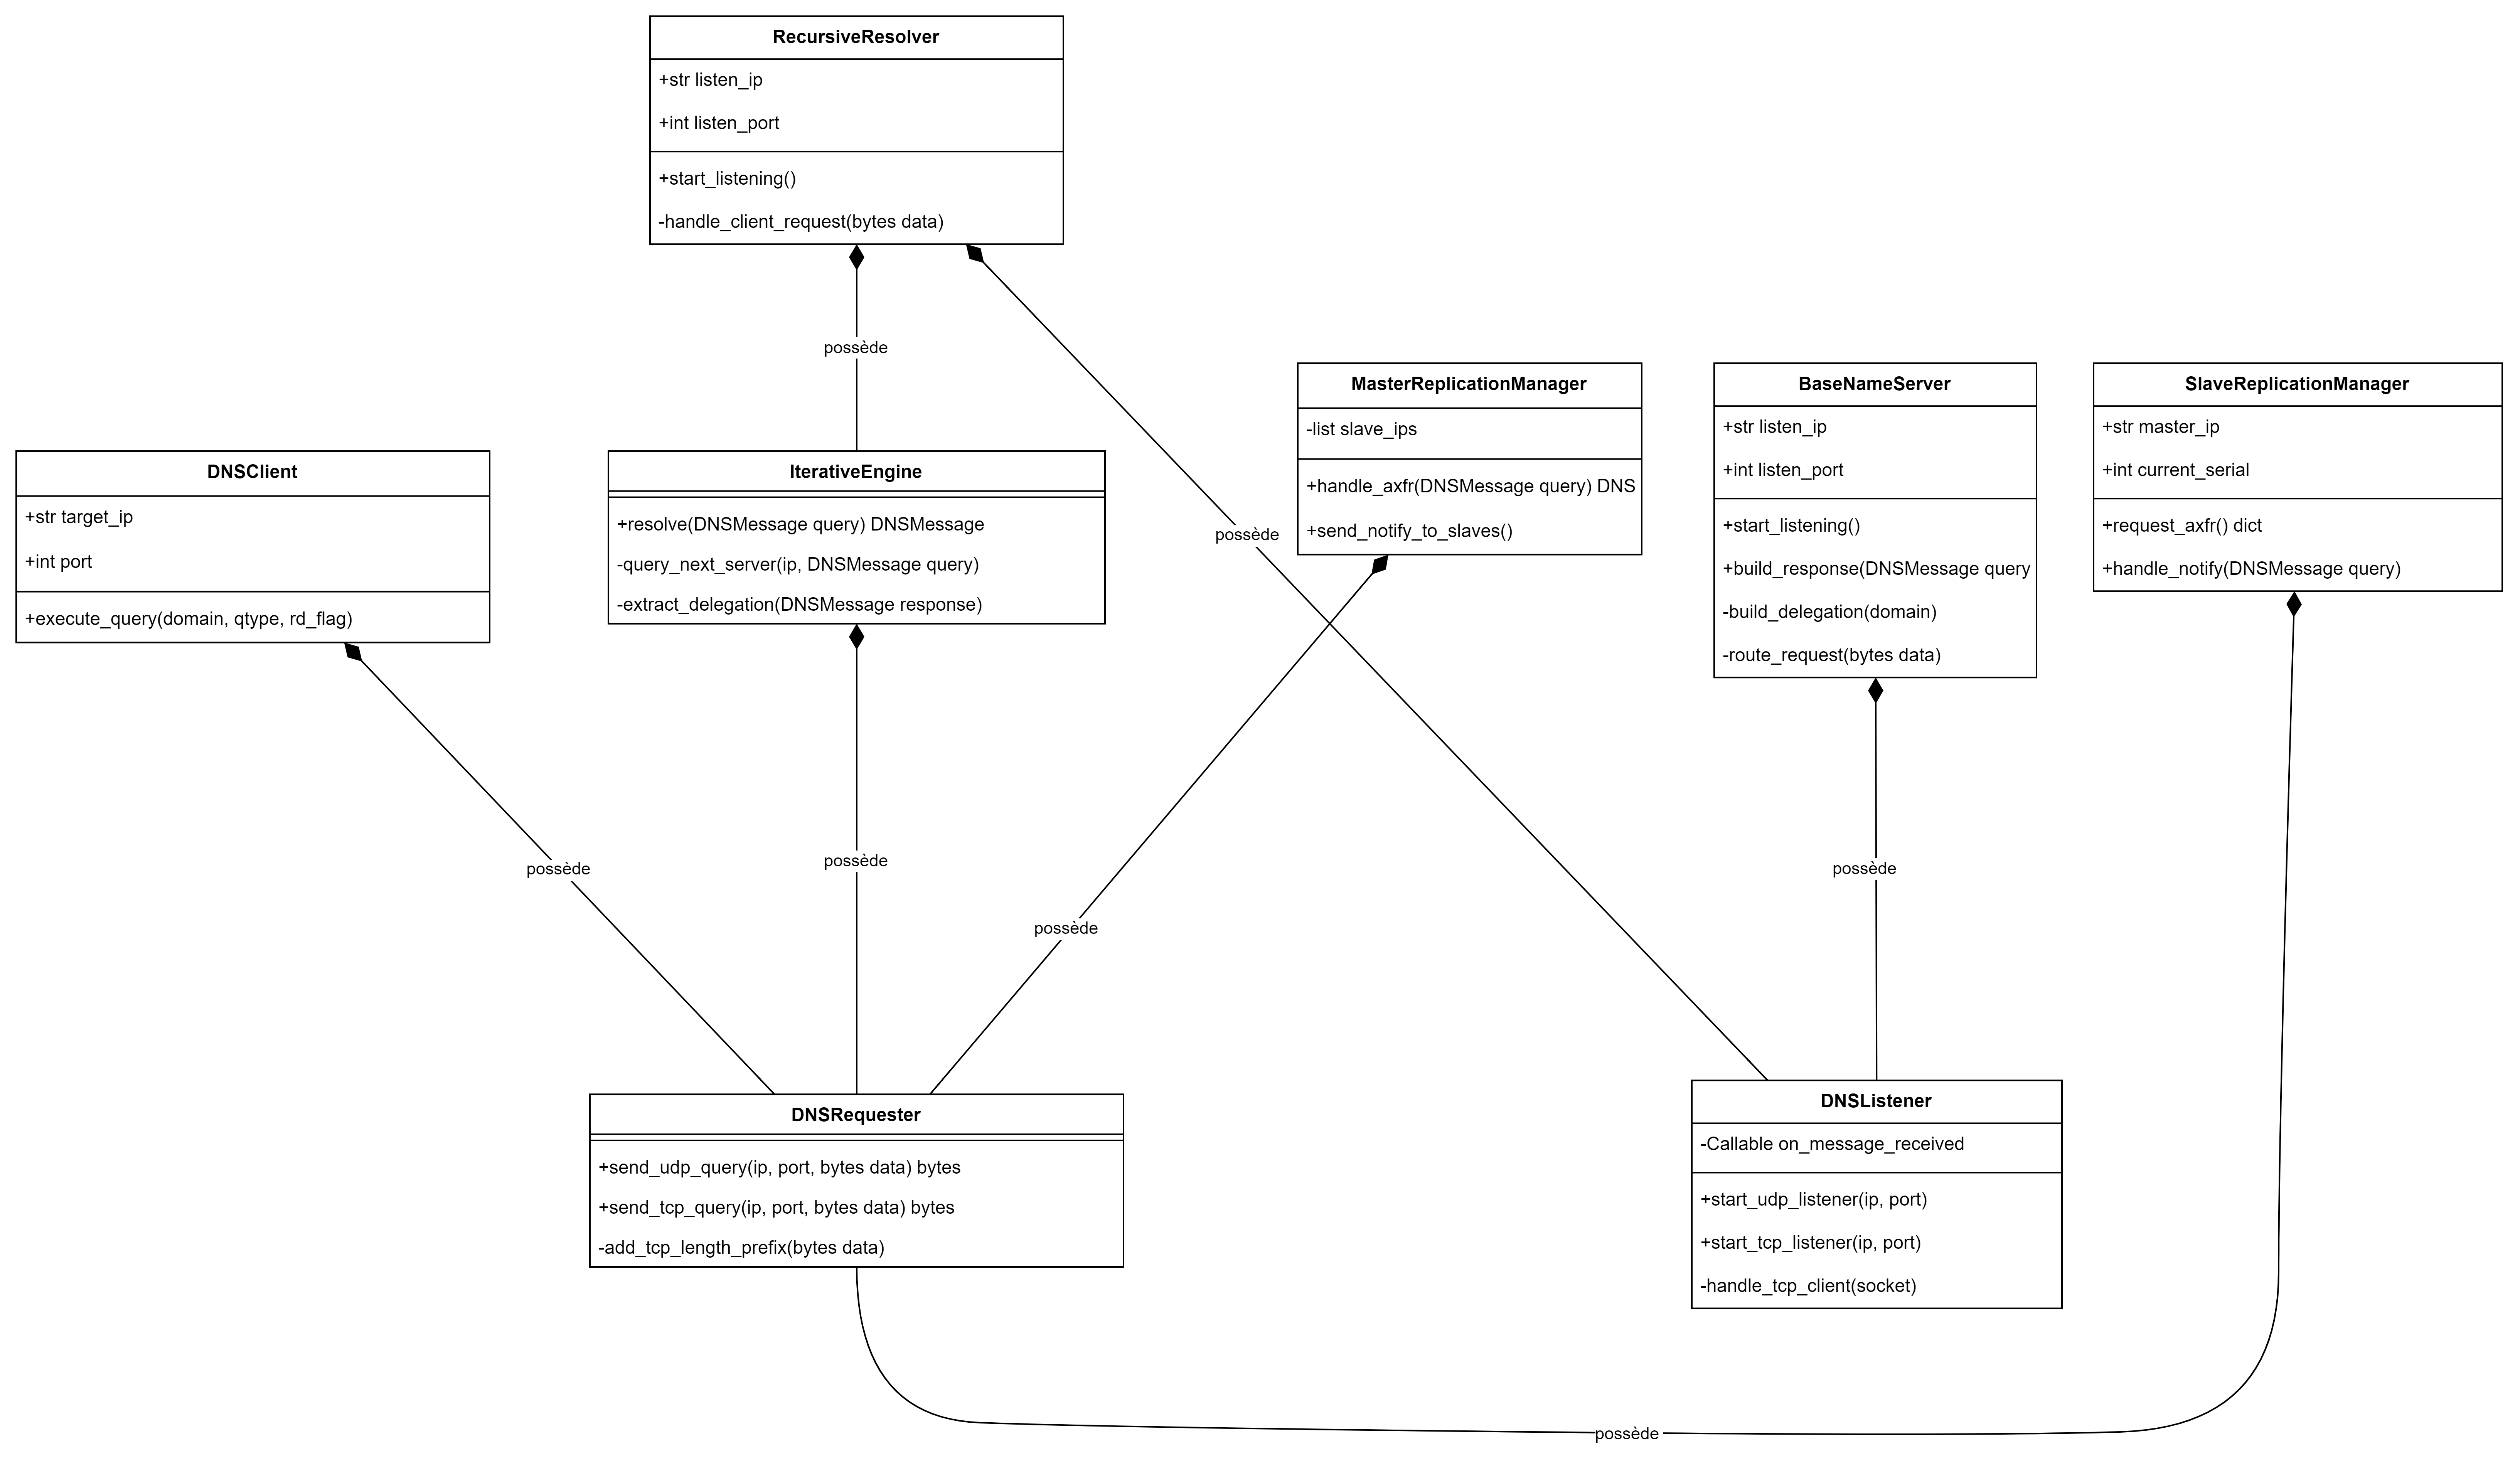
\includegraphics[width=15cm]{figures/technique/class_reseau.png}
    \caption{Diagramme de classes de l'architecture réseau.}
    \label{fig:diagramme_classes_reseau}
\end{figure}
Comme illustré dans ce diagramme de classes, les classes \texttt{DNSListener} et \texttt{DNSRequester} sont utilisées par de nombreux composants du système.
Il est donc essentiel que ces classes soient génériques et indépendantes de la logique métier.

La classe \texttt{DNSListener} permet d'ouvrir un serveur d'écoute, TCP ou UDP, sur un port donné.
La réception des requêtes est entièrement gérée par cette classe.
Une fois la requête interceptée, elle est transmise à une fonction de rappel (\texttt{callback}) fournie par le composant appelant.
\begin{figure}[H]
    \centering
    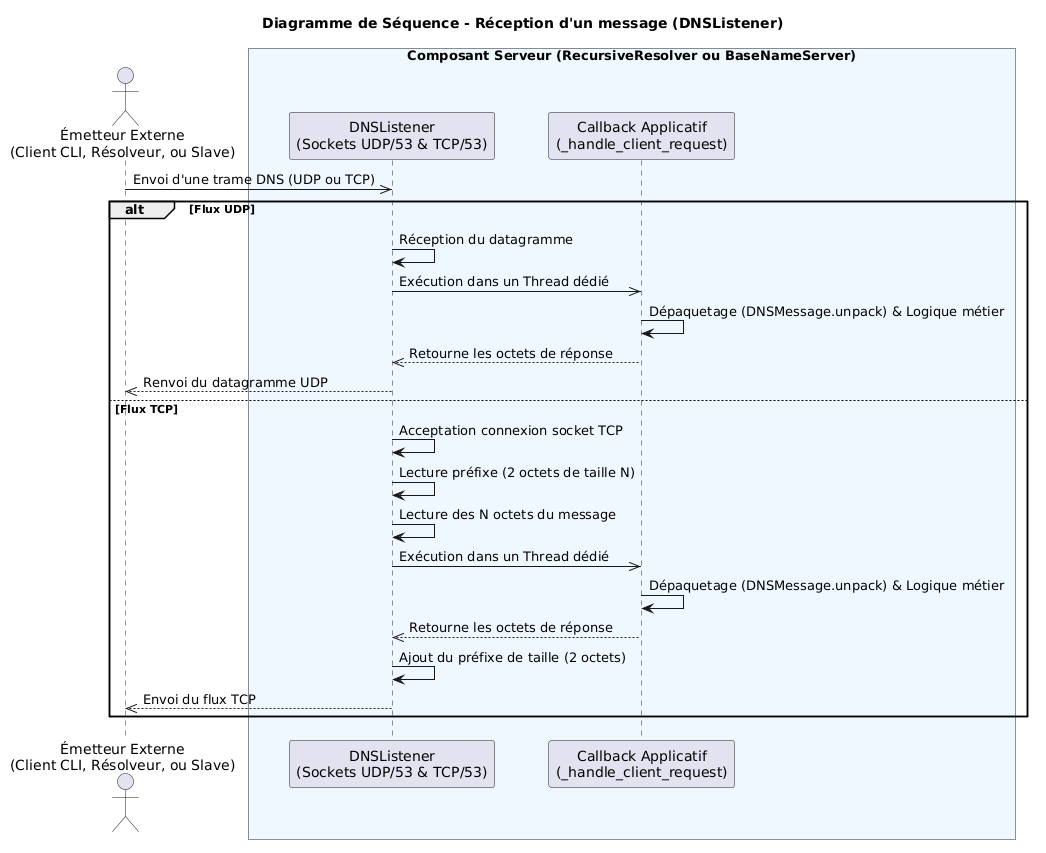
\includegraphics[width=15cm]{figures/technique/sequence_reseau_in.png}
    \caption{Séquence de communication pour les requêtes entrantes.}
    \label{fig:sequence_reseau_in}
\end{figure}

La classe \texttt{DNSRequester} permet d'envoyer des requêtes DNS TCP et UDP à un serveur distant.
Cette classe gère uniquement l'émission de la requête et la réception de la réponse.
C'est le composant appelant qui est responsable de la création de la requête au format binaire et de l'analyse de la réponse reçue.
Dans le cas d'une réponse tronquée, c'est le composant appelant qui décide de relancer la requête en TCP.
\begin{figure}[H]
    \centering
    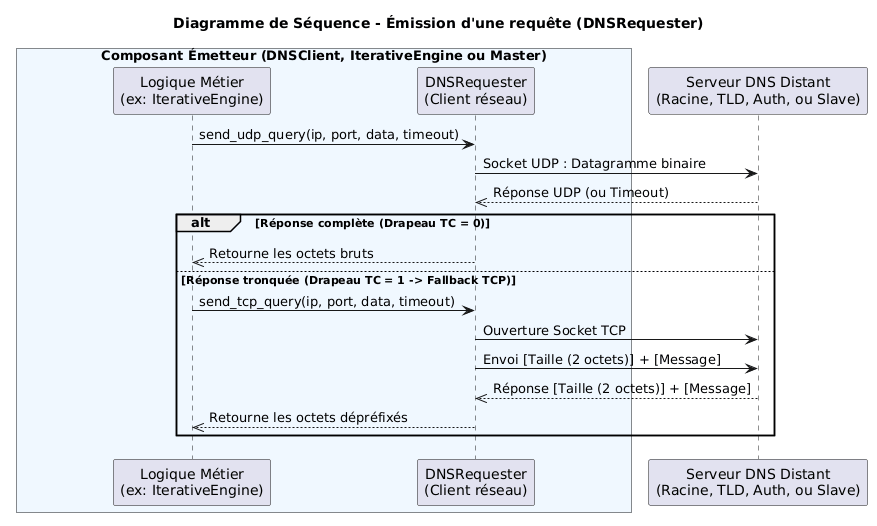
\includegraphics[width=15cm]{figures/technique/sequence_reseau_out.png}
    \caption{Séquence de communication pour les requêtes sortantes.}
    \label{fig:sequence_reseau_out}
\end{figure}

\subsection{Résolution DNS}
\begin{figure}[H]
    \centering
    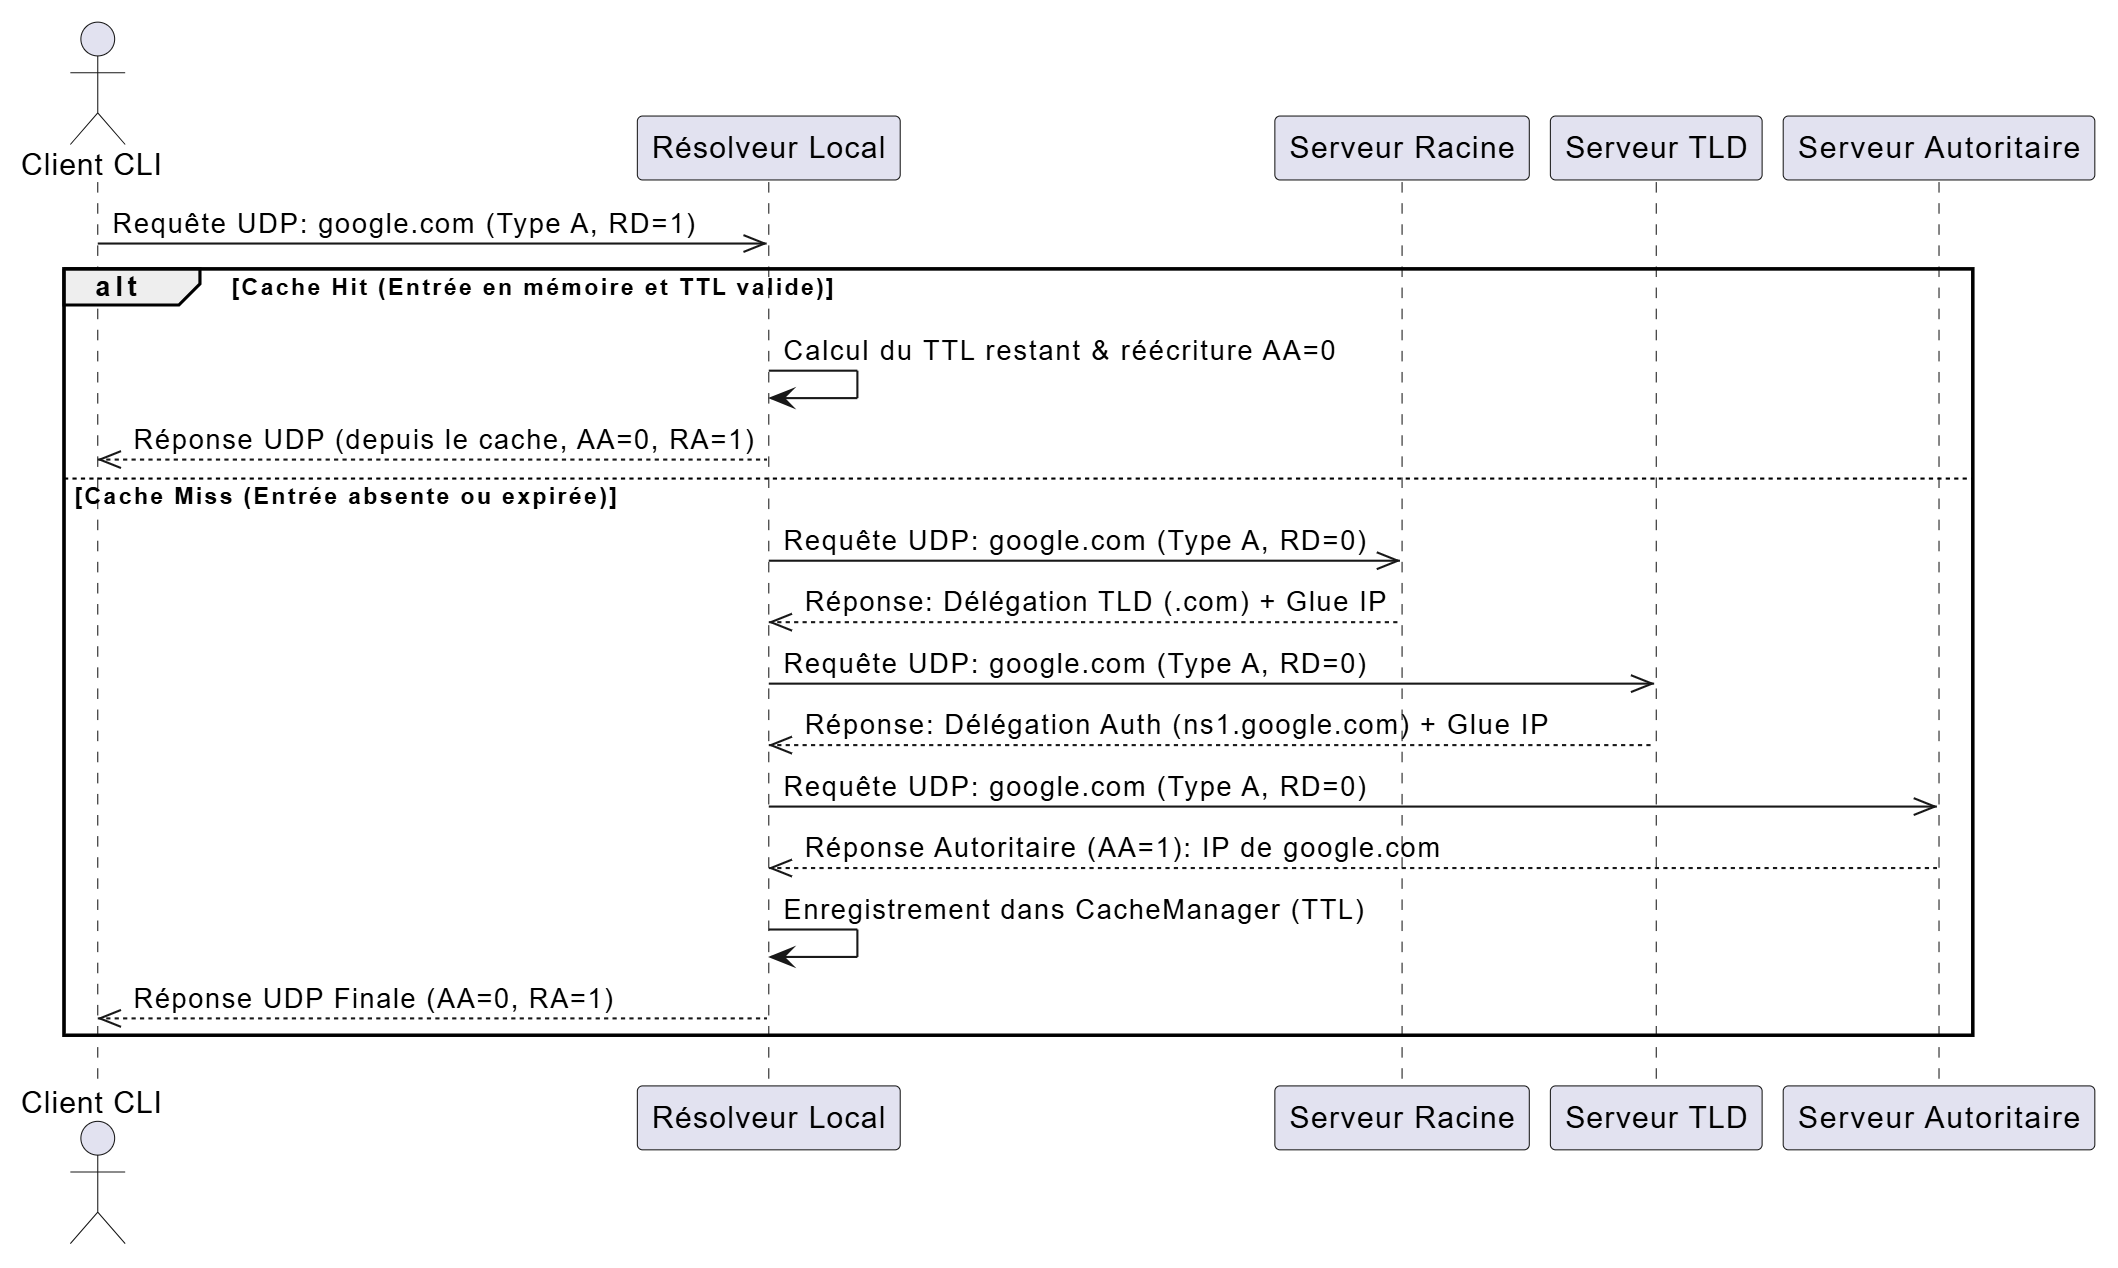
\includegraphics[width=15cm]{figures/technique/sequence_resolver.png}
    \caption{Diagramme de séquence de la résolution.}
    \label{fig:sequence_resolver}
\end{figure}

\subsubsection{Parcours d'une requête récursive}
% TODO: Détailler la boucle de résolution dans IterativeEngine.
% % [À MENTIONNER]: Analyse logique de la condition d'arrêt de la récursion : justification de l'utilisation d'opérateurs 'OR' (response.answers OR response.rcode != NOERROR OR response.aa == 1).
Le protocole DNS prévoit que l'information est répartie sur plusieurs serveurs de noms.
Trouver le serveur autoritaire pour un nom de domaine donné nécessite souvent plusieurs étapes.
Il faut d'abord interroger les serveurs Racines pour obtenir les serveurs de noms des TLD, puis interroger ces derniers pour obtenir les serveurs de noms spécifiques à la zone, et enfin interroger le serveur autoritaire pour obtenir la réponse finale.
La résolution récursive est le processus par lequel un résolveur DNS effectue ces étapes de manière transparente pour le client.

Le cœur de la résolution récursive réside dans la classe \texttt{IterativeEngine}.
Lorsqu'un client demande la résolution d'un nom de domaine avec le flag \texttt{RD=1} (\texttt{Recursion Desired}), le moteur entame une boucle itérative en interrogeant d'abord les serveurs Racines (\texttt{Root Hints}).
La logique repose sur l'analyse de la réponse à chaque itération.

La condition d'arrêt de cette boucle est régie par un opérateur logique \texttt{OU} (OR) vérifiant trois critères :
\begin{enumerate}
\item \texttt{response.answers} n'est pas vide : La réponse finale a été trouvée.
\item \texttt{response.rcode != 0} : Le serveur distant signale une erreur définitive (ex: NXDOMAIN, indiquant que le domaine n'existe pas).
\item \texttt{response.aa == 1} : Le serveur interrogé fait autorité sur la zone, même s'il ne renvoie pas de réponse (cas d'un \texttt{NODATA}, indiquant que le domaine existe mais pas pour le type demandé).
\end{enumerate}
Tant qu'aucune de ces conditions n'est remplie, le résolveur extrait les adresses IP (\texttt{Glue Records}) situées dans la section \texttt{Additional} de la réponse pour identifier le prochain serveur d'autorité à interroger (TLD, puis serveur de noms spécifique) et relance la boucle.

\subsubsection{Gestion du Cache}
% TODO: Expliquer l'expiration paresseuse ("Lazy Expiration") et le Negative Caching.
% % [À MENTIONNER]: Réécriture obligatoire du flag AA=0 à la volée lorsqu'une réponse est servie depuis le cache.
% % [À MENTIONNER]: Recalcul dynamique du TTL restant (remaining_ttl = expires_at - now) appliqué sur chaque ResourceRecord avant réémission.
Une résolution DNS récursive peut générer un grand nombre de requêtes et de réponses.
Il est donc nécessaire de stocker les réponses reçues pour éviter de surcharger le réseau avec des requêtes redondantes.
Un système de cache situé au niveau du résolveur récursif permet d'éviter cette surcharge.

Lorsque le résolveur récursif reçoit une requête, il vérifie si la réponse est déjà présente dans le cache.
Si c'est le cas, il renvoie la réponse directement au client sans interroger les serveurs de noms.
S'il n'y a pas de réponse stockée pour cette requête ou que cette dernière a expirée, le résolveur procède avec une résolution récursive classique.

Ce mécanisme permet de réduire le temps de réponse pour les clients et d'alléger la charge sur les serveurs de noms.
Cependant, en ne vérifiant pas les réponses au près d'une source autoritaire, il est possible que le cache contienne des informations obsolètes.
C'est pour cela que chaque enregistrement DNS possède un champ TTL (Time To Live) qui indique combien de temps il peut être conservé dans le cache avant d'être considéré comme périmé.
Le TTL est défini par l'administrateur de la zone et est transmis dans les réponses DNS.

Le système de cache est implémenté dans une classe indépendante pour garantir la modularité (il devient facile d'ajouter ce mécanisme à d'autres composants comme le client).
Cette classe, \texttt{CacheManager}, a comme attribut un dictionnaire et comme méthodes \texttt{store}, \texttt{retrive} et \texttt{clear\_cache}.
Le dictionnaire a comme clé une combinaison du nom de domaine et type de requête et comme valeur, un objet contenant le message de réponse sauvegardé pour cette requête et le temps d'expiration (TTL).
Si le résultat de la requête est une erreur (NXDOMAIN, SERVFAIL, REFUSED), il est également stocké dans le cache avec un TTL minimal (300s) pour éviter de répéter la même requête inutilement.

Les données du cache sont stockées en mémoire vive pour un accès rapide.
Cela implique que le cache est perdu à chaque redémarrage du résolveur récursif.
En effet, il n'y a pas de bénéfice à stocker les réponses dans un fichier sur le disque dur puisque le TTL des enregistrements est généralement très court (de quelques secondes à quelques heures) et que le cache se reconstruit rapidement à l'utilisation.

Lors du stockage, une copie profonde du message de réponse est ajoutée au dictionnaire avec le temps d'expiration calculé en ajoutant le TTL de la réponse au temps actuel lors du stockage.

Lors de la récupération, la validité de la réponse est vérifiée, son id est remplacé par celui de la requête et le flag AA est mis à 0 pour indiquer que la réponse provient d'un cache non autoritaire.
Le TTL restant doit également être recalculé en soustrayant le temps actuel du temps d'expiration.

Enfin, la méthode \texttt{clear\_cache} permet de vider le cache en supprimant toutes les entrées du dictionnaire.
Elle peut être déclenchée par le client en envoyant une requête de type \texttt{TXT} avec le nom de domaine \texttt{flush.cache.local}.


\subsection{Chargement de zones}
\begin{figure}[H]
    \centering
    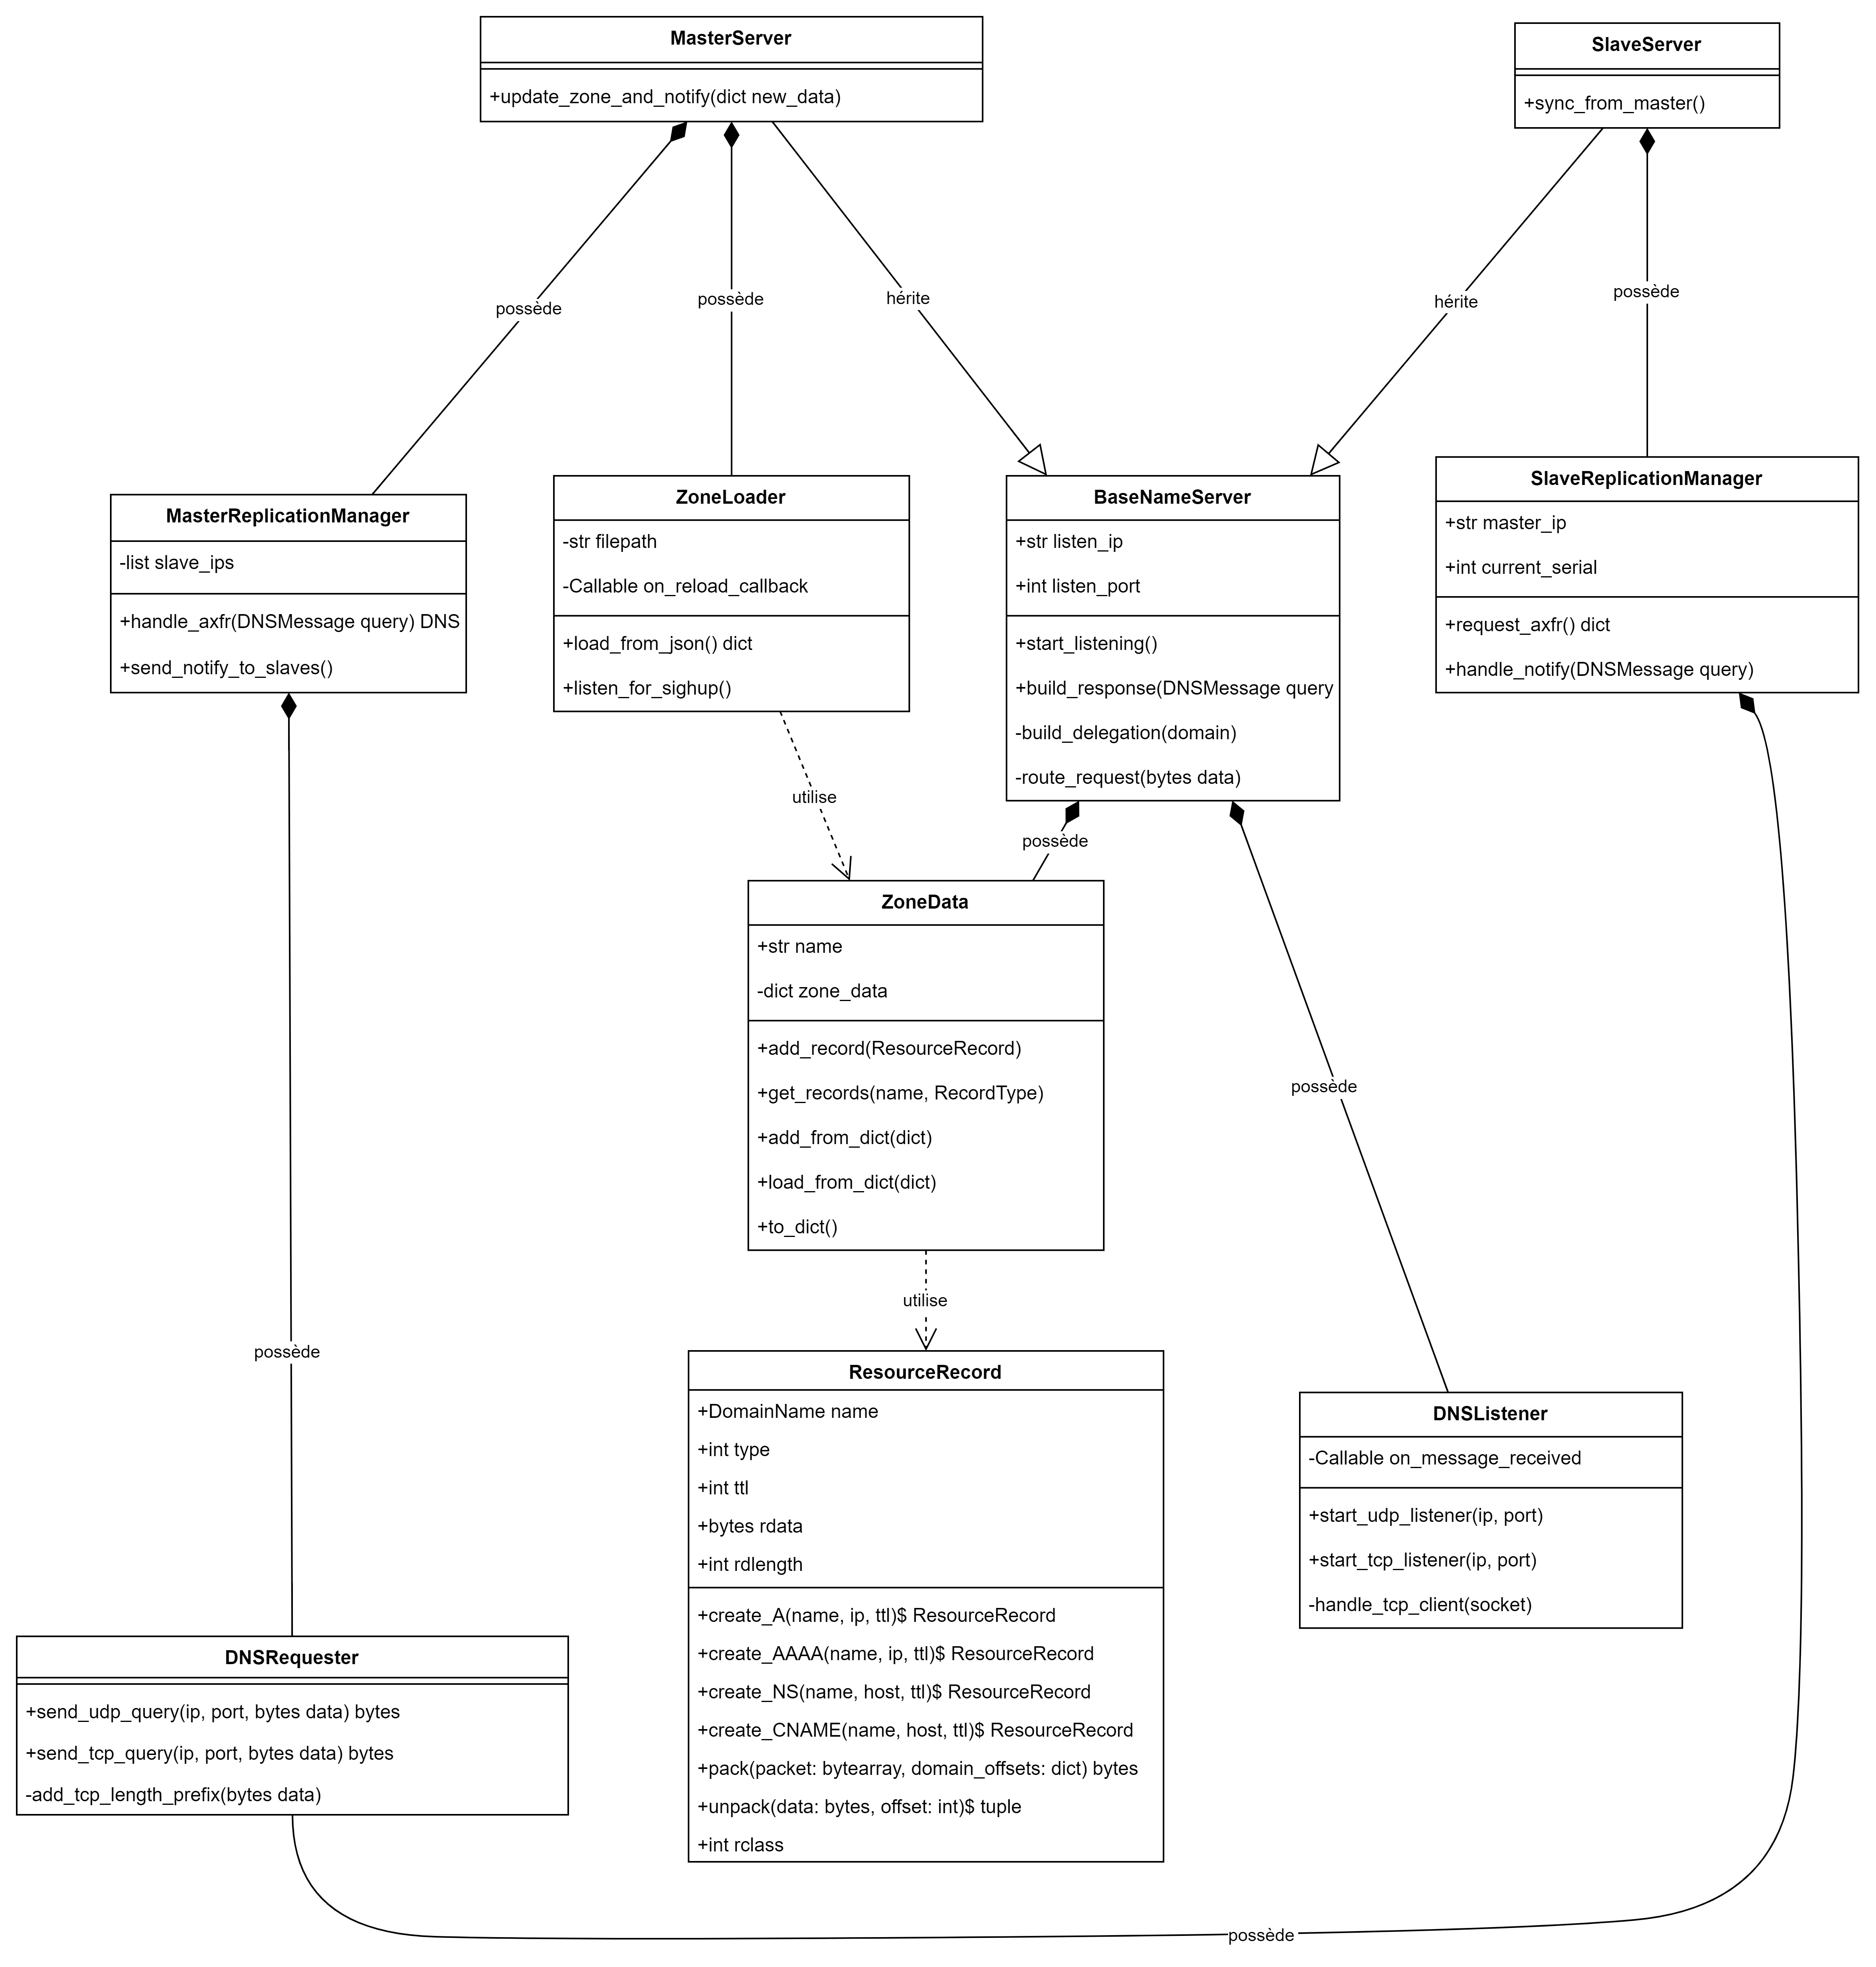
\includegraphics[width=15cm]{figures/technique/class_replication.png}
    \caption{Diagramme de classes du chargement de zones.}
    \label{fig:diagramme_classes_replication}
\end{figure}

\subsubsection{Stockage JSON}
% TODO: Justifier l'utilisation du format JSON en mémoire vive avec accès en O(1) par clé (Nom, Type).
Pour qu'un serveur de nom puisse répondre aux requêtes, il doit posséder les informations de la zone qu'il gère.
Alors que la norme historique (RFC 1035) préconise l'utilisation de fichiers de zone au format texte brut BIND (caractérisé par des directives telles que \texttt{\$ORIGIN} ou des notations relatives avec \texttt{@}), nous avons fait le choix de stocker les zones dans des fichiers au format JSON.

Le format retenu structure la zone sous la forme d'un dictionnaire imbriqué où chaque nom de domaine constitue une clé de premier niveau, associée à un sous-dictionnaire indexé par type d'enregistrement (\texttt{A}, \texttt{AAAA}, \texttt{NS}, \texttt{TXT}, etc.) :

\begin{verbatim}
{
  "be": {
    "NS": [
      {"host": "ns1.tld.be", "ttl": 86400}
    ]
  },
  "ns1.tld.be": {
    "A": [
      {"ip": "10.53.0.101", "ttl": 300}
    ]
  }
}
\end{verbatim}

Ce choix s'appuie sur plusieurs arguments techniques et pragmatiques :
\begin{itemize}
    \item \textbf{Simplicité et robustesse du parsing :} Le format BIND traditionnel nécessite l'écriture d'un analyseur syntaxique (\texttt{parser}) complexe pour gérer les retours à la ligne, les directives relatives et les commentaires. À l'inverse, le format JSON est nativement pris en charge par le module \texttt{json} de la bibliothèque standard de Python. Son chargement est immédiat et évite d'introduire des bogues de lecture sur le serveur.
    \item \textbf{Adéquation avec la structure en mémoire :} La hiérarchie du fichier JSON reflète exactement la structure de données interne utilisée par notre classe \texttt{ZoneData}. Cette correspondance directe permet d'instancier les objets \texttt{ResourceRecord} sans transformation lourde et garantit des recherches d'enregistrements en temps constant $\mathcal{O}(1)$ grâce aux tables de hachage.
    \item \textbf{Indépendance vis-à-vis de l'interopérabilité réseau :} Le fichier de zone est un composant strictement local et interne au serveur d'autorité. Son format sur disque n'impacte en rien le protocole réseau : toutes les trames échangées avec l'extérieur (UDP et TCP) respectent scrupuleusement la norme binaire RFC 1035. Les clients standards (\texttt{dig}, \texttt{nslookup}) ou les résolveurs tiers interagissent avec le serveur sans jamais avoir connaissance du format de stockage interne.
    \item \textbf{Évolutivité via la classe ZoneData :} La gestion du stockage est entièrement isolée au sein de la classe \texttt{ZoneData}. Si une compatibilité avec les fichiers de zone BIND historiques s'avérait nécessaire à l'avenir, il suffirait d'ajouter une méthode de traduction/parsing BIND dans cette classe sans devoir modifier le moteur du serveur ni le reste de l'architecture.
\end{itemize}

\subsubsection{Rechargement à chaud et surveillance de fichier}
% TODO: Expliquer l'évolution de l'architecture du rechargement.
% % [À MENTIONNER]: Abandon de l'interception SIGHUP (non supportée sous Windows) au profit d'un thread d'arrière-plan de surveillance par polling du mtime (os.path.getmtime).
Afin de répondre au besoin de continuité de service (US-3.6), le serveur d'autorité doit pouvoir intégrer des modifications de la zone DNS sans nécessiter un redémarrage du processus.
Initialement, cette fonctionnalité a été pensée autour de l'interception du signal UNIX \texttt{SIGHUP} via le module \texttt{signal}.
Cependant, ce signal n'étant pas nativement supporté par le système d'exploitation Windows, une approche plus universelle a été adoptée pour garantir la portabilité du code.
L'architecture finale repose sur un thread d'arrière-plan (\texttt{background thread}) exécutant une boucle de \texttt{polling}.
Ce thread interroge périodiquement les métadonnées du fichier de zone via \texttt{os.path.getmtime()} pour détecter un changement de date de modification.
Si une altération est détectée, le fichier est rechargé, le dictionnaire en RAM est écrasé de manière \texttt{thread-safe} (utilisant un verrou de synchronisation), et une notification de mise à jour est déclenchée.

\subsubsection{La Réplication Master / Slave et Rechargement}
% TODO: Détailler le workflow de réplication secondaire.
% % [À MENTIONNER]: Format du transfert AXFR : Choix entre le raccourci applicatif JSON encapsulé dans le RDATA du type 252 et l'alignement RFC (flux d'enregistrements binarisés encadré par le SOA).
Pour assurer la redondance et la tolérance aux pannes (Épic 4), un mécanisme de réplication a été implémenté entre un serveur \texttt{Master} et des serveurs \texttt{Slaves}.
Dès que le serveur Master détecte une modification de sa zone, il émet une trame UDP avec l'OpCode \texttt{NOTIFY} (4) à destination de ses Slaves.
À la réception de ce signal, le Slave initie une connexion TCP pour demander un transfert de zone complet (requête de type \texttt{AXFR}, QTYPE 252).

La norme RFC 1996~\cite{rfc1996} décrit traditionnellement le transfert AXFR comme un flux séquentiel de multiples enregistrements binaires encadré par des enregistrements SOA.
Cependant, étant donné que notre écosystème stocke nativement les zones au format JSON, nous avons opté pour une approche pragmatique et simplifiée.
Le serveur Master sérialise l'intégralité du dictionnaire JSON en une seule chaîne de caractères encodée en UTF-8, et l'encapsule dans la section \texttt{RDATA} d'un unique enregistrement de type 252.
Le Slave reçoit cette trame TCP, extrait le JSON, et met à jour sa mémoire instantanément.
Cette méthode respecte l'encapsulation DNS tout en tirant pleinement parti des structures de données de notre implémentation.

\begin{figure}[H]
    \centering
    \includegraphics[width=15cm]{figures/technique/sequence_replication.png}
    \caption{Diagramme de séquence de la réplication.}
    \label{fig:diagramme_de_sequence_replication}
\end{figure}


\subsection{Conception des classes}
% TODO: Présenter les choix de composition vs héritage.
% - Insérer le Diagramme de Classes final complet.
Ce diagramme de classes présente l'ensemble des classes implémentées dans le projet.
\begin{figure}[H]
    \centering
    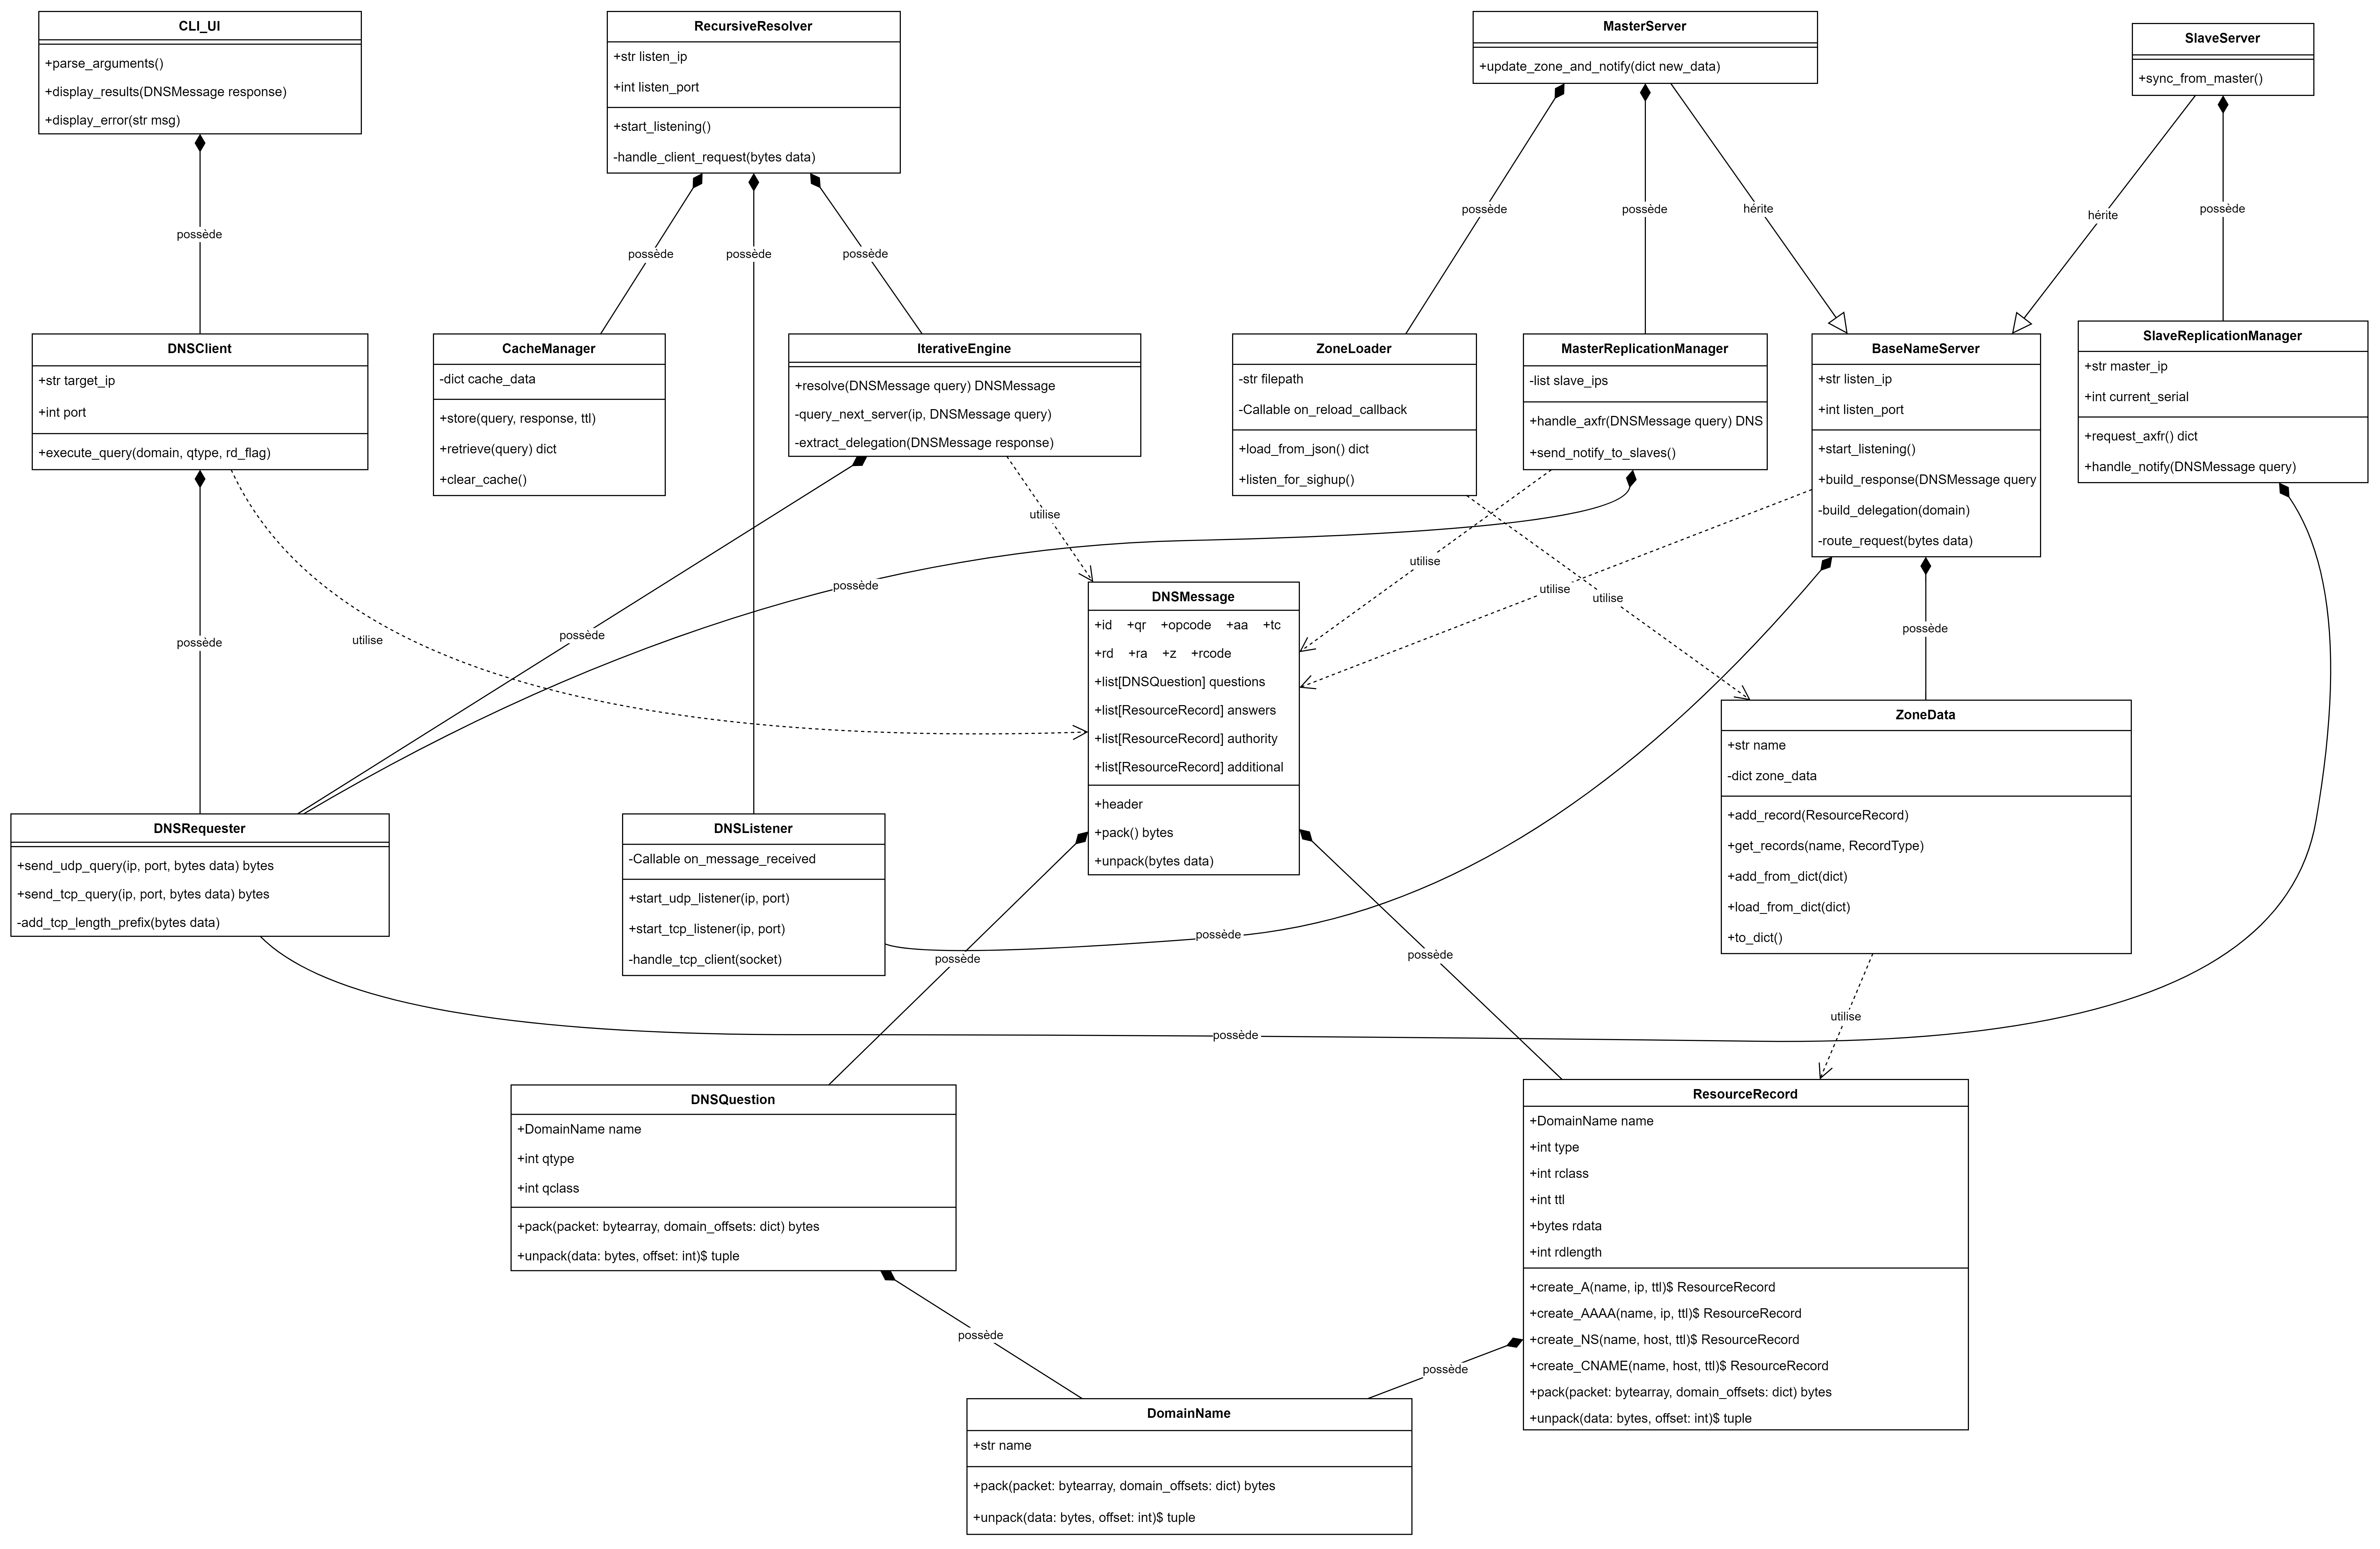
\includegraphics[width=15cm]{figures/technique/class.png}
    \caption{Diagramme de classes.}
    \label{fig:diagramme_classes}
\end{figure}

\section{Implémentation}
\subsection{Arborescence du Projet}
% TODO: Insérer et expliquer l'arborescence des dossiers (core/, name_server/, recursive_resolver/, client/, tests/).

\subsection{Qualité et Tests (TDD)}
% TODO: Présenter la suite de tests automatisée.
% - Utilisation de pytest pour exécuter les 39+ tests unitaires.
% - Utilisation de unittest.mock pour simuler l'environnement réseau et les timestamps (time.time).
% % [À MENTIONNER]: Stratégie de test des threads d'arrière-plan (mocking de os.path.getmtime et os.utime pour simuler les modifications de fichiers de zone).

\subsection{Déploiement sous Docker}
% TODO: Expliquer l'orchestration multi-conteneurs.
% - Configuration du réseau Docker statique (10.53.0.0/16) indispensable pour fixer l'IP des serveurs autoritaires et des Glue Records.
% - Utilisation de PYTHONUNBUFFERED=1 pour le suivi temps réel des logs.
% % [À MENTIONNER]: Le piège des Inodes Docker : Résolution du bug de rechargement en montant le répertoire parent (../zones:/app/zones) plutôt que des fichiers isolés pour préserver la liaison d'inode lors des sauvegardes atomiques de l'hôte.
% % [À MENTIONNER]: Procédure d'interrogation et configuration de nslookup pour le débogage (passage obligatoire par le mode interactif : 'set port=10054', 'server 127.0.0.1').

\subsection{Refactoring et Retours d'Expérience de Terrain}

\subsubsection{Capsules typées et gestion de la mémoire}
% TODO: Expliquer la transition des structures dictionnaires vers des objets typés (DNSQuestion, ResourceRecord, DNSMessage).
% - Utilisation de copy.deepcopy() dans le cache manager pour prévenir la corruption des objets partagés entre requêtes.

\subsubsection{Bugs critiques identifiés et résolus}
% TODO: Retour sur les corrections majeures lors du développement.
% % [À MENTIONNER]: Le bug du typage Enum : Correction des échecs de comparaison silencieux entre String ("NS") et RecordType.NS dans la recherche de délégations de ZoneData.
% % [À MENTIONNER]: Le piège de la référence mémoire lors du hot-reload : Mise à jour in-place de l'instance ZoneData existante via load_from_dict() au lieu de réinstancier l'objet (ce qui brisait la référence détenue par le moteur AuthoritativeEngine).
\section{Analyse retrospective}
\subsection{Bilan des résultats}
% TODO: Évaluer l'atteinte des objectifs.
% - Conformité validée avec la RFC 1035.
% - Validation des scénarios de résolution complète de bout en bout (Client -> Résolveur -> Root -> TLD -> Auth).

\subsection{Limites et perspectives d'améliorations}
% TODO: Identifier les axes d'évolution futurs.
% - Concurrence : Limites du modèle Thread-per-connection et opportunité d'une refonte asynchrone avec asyncio.
% - Support protocolaire : Gestion complète des extensions EDNS0 et des gros paquets UDP (PATH MTU).
% - Persistance : Persistance sur disque du cache DNS pour éviter le démarrage à froid.
% - Sécurité : Implémentation de la validation DNSSEC (signatures cryptographiques RRSIG/DNSKEY).
\section*{Conclusion}
L'objectif du projet était de concevoir un environnement DNS complet, en partant de zéro et en utilisant uniquement la bibliothèque standard Python et en respectant la méthode \textit{Agile}.

Le cahier des charges est rempli. L'architecture orientée objet mise en place permet à chaque serveur d'agir simultanément comme autorité sur une zone, résolveur récursif et gestionnaire de cache.

L'implémentation a été validée par une suite de tests unitaires et d'intégration automatisés. La conformité avec la RFC 1035 a été vérifiée via des outils d'administration standards (\texttt{dig}), démontrant l'interopérabilité du code au sein de l'infrastructure Docker simulée.
\section*{Déclaration d'usage de l'IA générative}
Conformément au Guide du Projet Innovant de l'Hénallux, je déclare avoir utilisé le grand modèle linguistique Gemini (Google) en tant qu'assistant à la rédaction lors de ce projet.
Son usage s'est limité à la reformulation académique de textes préalablement rédigés par mes soins, la mise en forme du code \textit{latex}, l'aide à la structuration des sections du rapport et l'aide à la rédaction des commentaires de certains schémas réalisés par mes soins.
L'entièreté de la réflexion, des choix techniques et de l'analyse sont le fruit de mon travail personnel.

Google, "Gemini," May 2024. Large language model. Available: https://gemini.google.com/

\subsection{Usages spécifiques}
Le même modèle a été utilisé pour la rédaction des fichiers de zones de test à partir du prompt suivant :
\begin{verbatim}
    Donne moi des beaux fichiers de zone pour les tests

exemple (juste pour te montrer le format):
{
  "www.test.be": {
    "A": [
      {"ip": "192.168.99.99", "ttl": 300}
    ]
  },
  "api.test.be": {
    "A": [
      {"ip": "192.168.99.100", "ttl": 300}
    ]
  },
  "mail.test.be": {
    "A": [
      {"ip": "192.168.99.101", "ttl": 300}
    ]
  },
  "www.example.be": {
    "A": [
      {"ip": "192.168.99.102", "ttl": 300}
    ]
  },
  "mail.example.be": {
    "A": [
      {"ip": "192.168.99.103", "ttl": 300}
    ]
  },
  "test.be": {
    "NS": [
      {"host": "ns1.test.be", "ttl": 86400}
    ]
  },
  "example.be": {
    "NS": [
      {"host": "ns1.test.be", "ttl": 86400}
    ]
  },
  "ns1.test.be": {
    "A": [
      {"ip": "10.53.0.102", "ttl": 300}
    ]
  }
}
\end{verbatim}

Il a également été utilisé pour la retranscription de code \textit{Python} en code \textit{PlantUML} de diagramme d'activité à partir du prompt suivant :
\begin{verbatim}
Fais des diagrammes d'action illustrant le routage (_route_request) et la résolution récursive avec le querynext hop
Illustre le mécanisme d'héritage et le fonctionnement de la méthode super
\end{verbatim}

Le code python lui a été fourni dans le prompt pour qu'il puisse générer les diagrammes d'action correspondants.


\nocite{*}
\bibliography{bibliographie}
\listoffigures

\end{document}